%!TEX program = lualatex
\documentclass[aspectratio=169]{beamer}

\usepackage{blindtext}
\usepackage{multimedia}

\usetheme{AVThesis}

\title{The Art of Robotics:\\\vspace{0.2em}\huge{Toward A Holistic Approach}}
\subtitle{Master of Science in Robotics\\Thesis Defense}
\author{Alexander Volkov Jr.}
\date{July 31, 2018}

% Change frame margins
\addtobeamertemplate{frametitle}{\vspace*{1cm}}{\vspace*{0cm}}

\setcounter{showSlideNumbers}{1}

\begin{document}
	\setcounter{showProgressBar}{0}
	\setcounter{showSlideNumbers}{0}

	\frame{\titlepage}

	\begin{frame}
		\frametitle{Talk Agenda}
		\begin{enumerate}
			\setlength{\itemsep}{4mm}
			\item Background
				\textcolor{AVThesisGrey}{\footnotesize\hspace{1em} How I ended up here.}
				
			\item Other Things
				\textcolor{AVThesisGrey}{\footnotesize\hspace{1em} Warm up the crowd with a quick review of some other things I've done.}
			
			\item The Big Picture
				\textcolor{AVThesisGrey}{\footnotesize\hspace{1em} Cover the central themes of this talk.}
			
			\item A Unifying Framework
				\textcolor{AVThesisGrey}{\footnotesize\hspace{1em} An old framework, revived.}
			
			\item Brushless PMSM Motors
				\textcolor{AVThesisGrey}{\footnotesize\hspace{1em} Operating limits, thermal management, liquid cooling.}
	
			\item Touching Robots
				\textcolor{AVThesisGrey}{\footnotesize\hspace{1em} Tactile sensing, contact modeling, whiskers, robot pain.}
			
			\item Conclusions
				\textcolor{AVThesisGrey}{\footnotesize\hspace{1em} Review key points and propose some future work.}
			
			\item Questions
				\textcolor{AVThesisGrey}{\footnotesize\hspace{1em} \emph{``Please clap...''}}
		\end{enumerate}
	\end{frame}

	\setcounter{framenumber}{0}
	\setcounter{showProgressBar}{1}
	\setcounter{showSlideNumbers}{1}
	
	\section{Background}
		\begin{frame}
			\frametitle{How I Ended Up Here}
		
		\end{frame}

	\section{Other Things}
		\begin{frame}
			\frametitle{Teaching with CMU's Gelfand Outreach Center}
			\begin{tikzpicture}[overlay, remember picture]
				\node[anchor=center] (gelfand-logo) at (0.88\textwidth, 0) {
\includegraphics[width=5cm]{media/gelfand-logo.jpg}};
			\end{tikzpicture}
			\begin{itemize}
				\item Introduction to Robotics with the Finch Platform
					\begin{itemize}
						\item Each session is 5 days, 3 hrs/day
						\item 4\textsuperscript{th} and 5\textsuperscript{th} graders
						\item 1 session Summer 2017 + 2 sessions Summer 2018
					\end{itemize}
					\vspace{1em}
				
			\end{itemize}
		\end{frame}
	
		\begin{frame}
			\frametitle{Teaching with CMU's Gelfand Outreach Center}
			\begin{tikzpicture}[overlay, remember picture]
				\node[anchor=center] (gelfand-logo) at (0.88\textwidth, 0) {
\includegraphics[width=5cm]{media/gelfand-logo.jpg}};
			\end{tikzpicture}
			\begin{itemize}
				\item Saturday Series LEGO WeDo Robotics
				\begin{itemize}
					\item 3 hour course
					\item 2\textsuperscript{nd} and 3\textsuperscript{rd} graders
					\item 1 session Spring 2018
				\end{itemize}
			\end{itemize}
		\end{frame}
		
		\begin{frame}
			\frametitle{Robotics Institute Meme Facebook Page}
			\begin{tikzpicture}[overlay, remember picture]
				\node[anchor=center] (ri-meme-screenshot) at (current page.center) {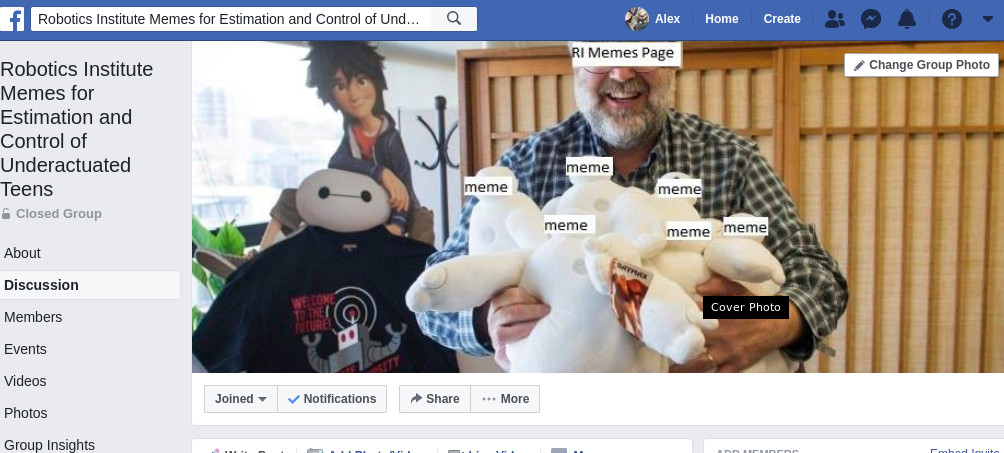
\includegraphics[width=\textwidth]{media/ri-memes.jpg}};
			\end{tikzpicture}
		\end{frame}
	
		\begin{frame}
			\frametitle{Robotics Institute Meme Facebook Page}
			\begin{itemize}
				\item Some statistics:
					\begin{itemize}
						\item The RI's first and only meme page
						\item Formed in March 2018
						\item 170 members
						\item 30 memes, 23 original contributions!
					\end{itemize}
			\end{itemize}
	\end{frame}
	
	\section{The Big Picture}
		\begin{frame}
			\frametitle{Breadth First}
			\begin{enumerate}
				\item 
			\end{enumerate}
		\end{frame}
	
			\begin{frame}
				\frametitle{Tangential Projects}
				Kruskal count + quadruped gaits
			\end{frame}

	\section{A Unifying Framework}
		\begin{frame}
			\frametitle{The Port-Hamiltonian Framework}
			\begin{itemize}
				\item Port-based Analysis
				\item Hamiltonian Dynamics
					\begin{itemize}
						\item 
					\end{itemize}
				\item
			\end{itemize}
		\end{frame}
	
		\begin{frame}
			\frametitle{Bond Graphs}
			
		\end{frame}

		\begin{frame}
			\frametitle{Hamiltonian Dynamics}
			
		\end{frame}

		\begin{frame}
			\frametitle{Putting it All Together}
			
		\end{frame}
	
	\section{Brushless PMSM Motors}
		
		\begin{frame}
			\frametitle{???}
		\end{frame}
	
	\section{Touching Robots}
	
		\begin{frame}
			\frametitle{The Most Important Sensory Modality}
		\end{frame}
	
		\begin{frame}
			\frametitle{Contact Models}
		\end{frame}
		
		\begin{frame}
			\frametitle{Terminator 2 Got It Right}
			\begin{center}
			\movie[height = 0.6\textwidth, width = 0.8\textwidth,showcontrols]{}{media/terminator2-pain.mp4}
			\end{center}
		\end{frame}

	\section{Closing Thoughts}
		\begin{frame}
			\frametitle{Closing Thoughts}
			\begin{itemize}
				\item Woo, Beamer!
			\end{itemize}
		\end{frame}
	
	\section{Questions?}
		
	
	\appendix
	\backupbegin
	  \begin{frame}
	    \frametitle{Backup slide 1}
	    \blindtext
	  \end{frame}
	\backupend

\end{document}
